% !TeX root = sta_paper.tex

Prior to data analysis, all trials containing invalid responses (0.1\% of trials) were removed, and trials with unusually long or short response times ($<200ms$ or $>3s$; 2\% of trials) were excluded. The overwhelming majority of these were too slow, possibly because participants took unscheduled breaks by deliberately delaying their response. Overall, 36,495 trials across the 15 participants remained for analysis. Descriptive statistics for task performance across conditions are summarized in Figure \ref{fig:descriptiveStats}. Overall accuracy is high in the set size 2 condition, as expected, and decreases as set size increases. In addition, Table \ref{tab:descriptiveStats} shows the mean hit and false alarm rates across all participants.

\begin{table}[ht]
{
\centering
\begin{tabular}{rrrrr}
  \hline
& \multicolumn{4}{c}{hits}\\
  \hline
& \multicolumn{2}{c}{simultaneous} & \multicolumn{2}{c}{sequential} \\
 set size & articulate & silent & articulate & silent \\ 
  \hline
  2 & 0.95 (0.022) & 0.95 (0.036) & 0.94 (0.026) & 0.94 (0.032) \\ 
  4 & 0.84 (0.065) & 0.88 (0.063) & 0.82 (0.076) & 0.82 (0.097) \\ 
  8 & 0.72 (0.079) & 0.70 (0.100) & 0.70 (0.101) & 0.70 (0.174) \\ 
  \hline
 & \multicolumn{4}{c}{false alarms}\\
  \hline
& \multicolumn{2}{c}{simultaneous} & \multicolumn{2}{c}{sequential}\\
set size & articulate & silent & articulate & silent \\ 
  \hline
  2 & 0.08 (0.040) & 0.06 (0.035) & 0.11 (0.066) & 0.07 (0.039) \\
  4 & 0.25 (0.131) & 0.22 (0.132) & 0.31 (0.166) & 0.26 (0.154) \\
  8 & 0.41 (0.120) & 0.39 (0.138) & 0.41 (0.142) & 0.42 (0.159) \\
\hline
\end{tabular}
}
\caption{Mean hit and false alarm rates for all conditions across all participants. Numbers in parentheses are standard deviations of the corresponding means.} 
\label{tab:descriptiveStats}
\end{table}

\begin{figure}[t]
 	\centering
	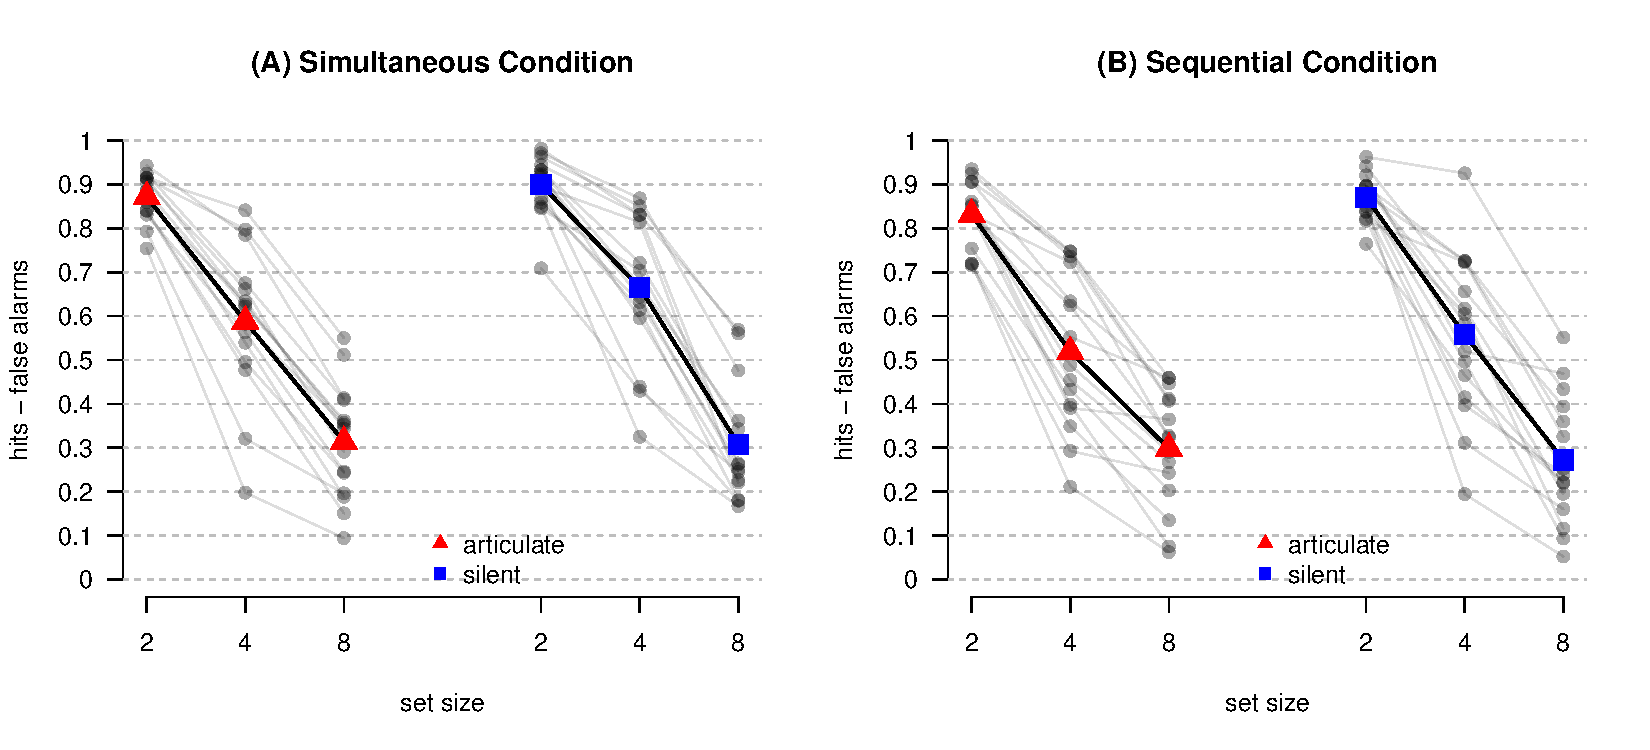
\includegraphics[width=\textwidth]{figures/descriptiveStats}
	\caption{Descriptive statistics for the relevant performance measure $d$ across the different conditions of the experiment. Semi-transparent black circles show the mean performance in each condition per participant and lines connect individual participants' means. Larger, colored symbols are group means for each condition, connected by thicker, black lines.}

	\label{fig:descriptiveStats}
\end{figure}


In order to assess the performance while controlling for response bias, for each condition-participant-set size combination we subtracted the false alarm rate from the hit rate to form an overall performance measure $d$ \citep{Cowan:etal:2005,Rouder:etal:2011}. Of particular interest is how the performance advantage for the silent condition is affected by the type of presentation. If participants verbalize when the presentation is sequential, we would predict that articulation would hurt performance much more with sequential presentation, and thus the advantage for the silent condition would be larger with sequential presentation. Figure~\ref{fig:effects}A plots the silent advantage in the simultaneous condition as a function of the same for the sequential condition for all participant by set size combinations. If participants were verbalizing, we would predict that many points would fall below the diagonal, indicating a greater advantage in the sequential condition. However, 27 out of the 45 points actually fall {\em above} the diagonal, inconsistent with the verbalization hypothesis. 

We also examined whether the apparent lack of an effect may be due to differences in strategy over the experimental sessions; however, a similar picture emerges when the effect is examined across the time, as in Figure~\ref{fig:effects}B. The verbalization hypothesis would predict that points would fall above the horizontal line at 0; on average; however, if anything, the points tend to fall {\em below} the line.

\begin{figure}[t]
 	\centering
	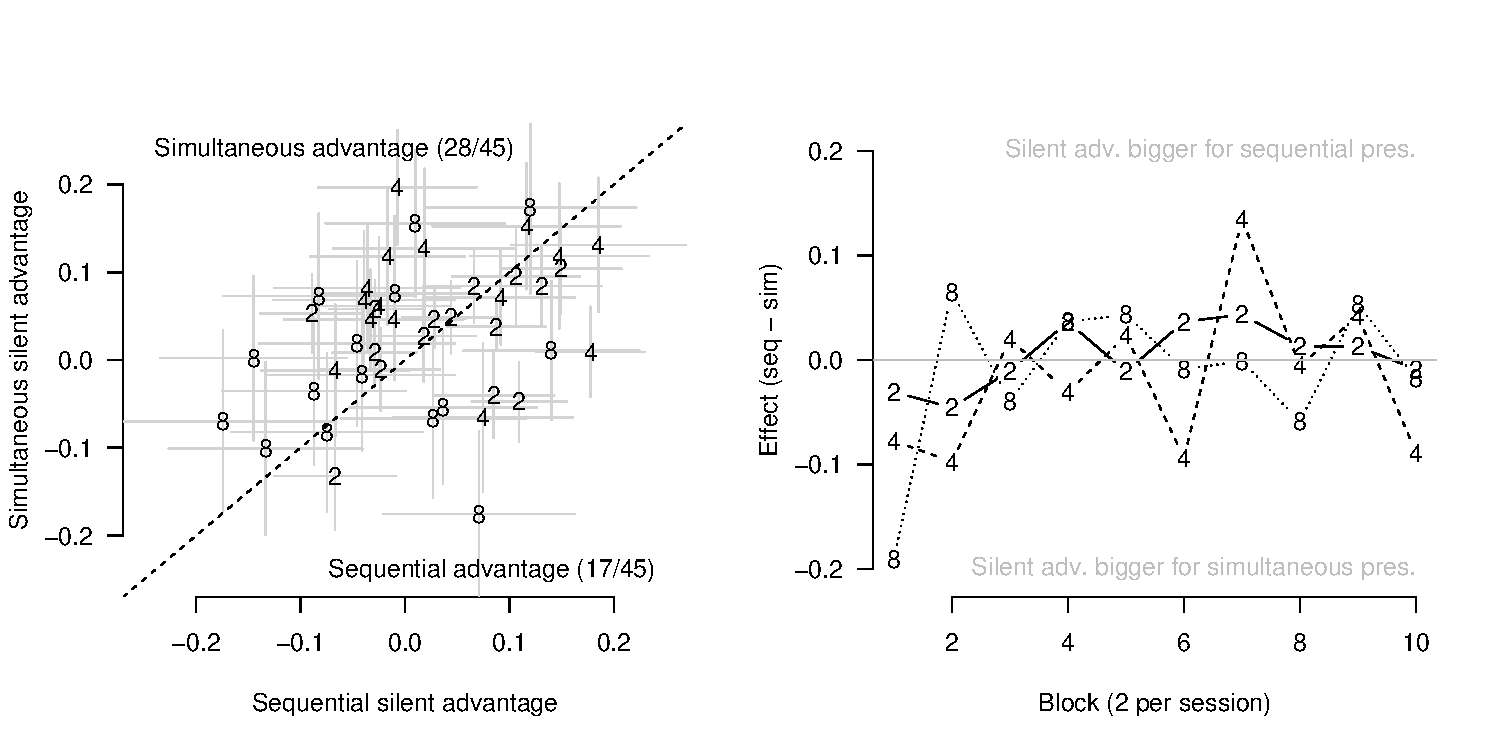
\includegraphics[width=\textwidth]{figures/effects}
	\caption{A: Advantage for silent condition (i.e., $d$ in silent condition minus $d$ in articulate condition) with simultaneous presentation as a function of the same for sequential presentation. Each point represents a single participant and set size. Error bars are approximate standard errors. B: The difference between the advantage for the silent condition in the sequential and simultaneous presentation conditions as a function of experimental block. In both plots, the number for each point represents the set size.}

	\label{fig:effects}
\end{figure}


\subsection{State-trace analysis}
Another way to examine whether there is any evidence for verbalization is a {\em state-trace analysis}. State-trace analysis, outlined in its original form by \citet{Bamber:1979}, is a data analysis technique intended to reveal how many latent dimensions a system requires to produce observed empirical results. A simple system may have only one latent dimension (e.g., memory capacity), and all experimental manipulations affect performance along that latent dimension. More complex systems may show relationships that are impossible to explain by a single dimension, and hence require positing more latent constructs. Considering visual change detection performance, one might imagine that only one latent dimension (e.g. visual memory capacity) or two latent dimensions (e.g. visual and verbal memory capacity) contribute to recognition accuracy. Articulatory suppression would only be necessary if there is an additional latent dimension that relies on verbal resources. That is, if visual change detection performance can be explained by a single latent dimension then articulatory suppression is not needed. To see whether a single latent dimension is supported, it is necessary to compare typical visual change detection accuracy to detection accuracy in a situation where verbal recoding would be especially beneficial, and compare the effect of preventing verbal recoding across these scenarios. 

In the logic of state-trace analysis, performance in the sequential and simultaneous presentation conditions arise from either one or more latent constructs. If they both arise from a single latent variable, such as working memory capacity --- and if performance in both is a monotone function of the latent variable -- then performance in the sequential presentation must be a monotone function of performance in the simultaneous condition. To the extent to which no monotone function can describe the relationship between simultaneous and sequential task performance, two latent constructs --- perhaps visual and verbal working memory capacity --- are assumed to be needed to describe the performance.

For the state-trace analysis, we again used $d$, the hit rate minus the false alarm rate, as a measure of performance. To reduce possibly spurious deviations we computed Bayesian estimates of $d$ under three reasonable constraints: first, we assumed that the true hit rate was greater than the true false alarm rate, and thus performance was truly above chance. Second, for both the sequential and the simultaneous condition, $d$ must decrease with increasing array set size; for instance, true $d$ to a set size of 8 cannot be better than performance to set size 4, all other things being equal. Third, it was assumed that suppression cannot benefit performance; for each set size and presentation condition, the true $d$ in the articulate condition must be less than in the silent condition. This restriction was applied because a small dual-task cost appearing in all conditions would be consistent within any working memory theory, and with our stimuli and meaningless articulation instructions, no benefit of articulation was reasonably expected. Estimating the true discrimination under these restrictions yields a less error-prone measure of performance due to the exclusion of implausible data patterns. 

%%% full-page figure
\begin{figure}
 	\centering
	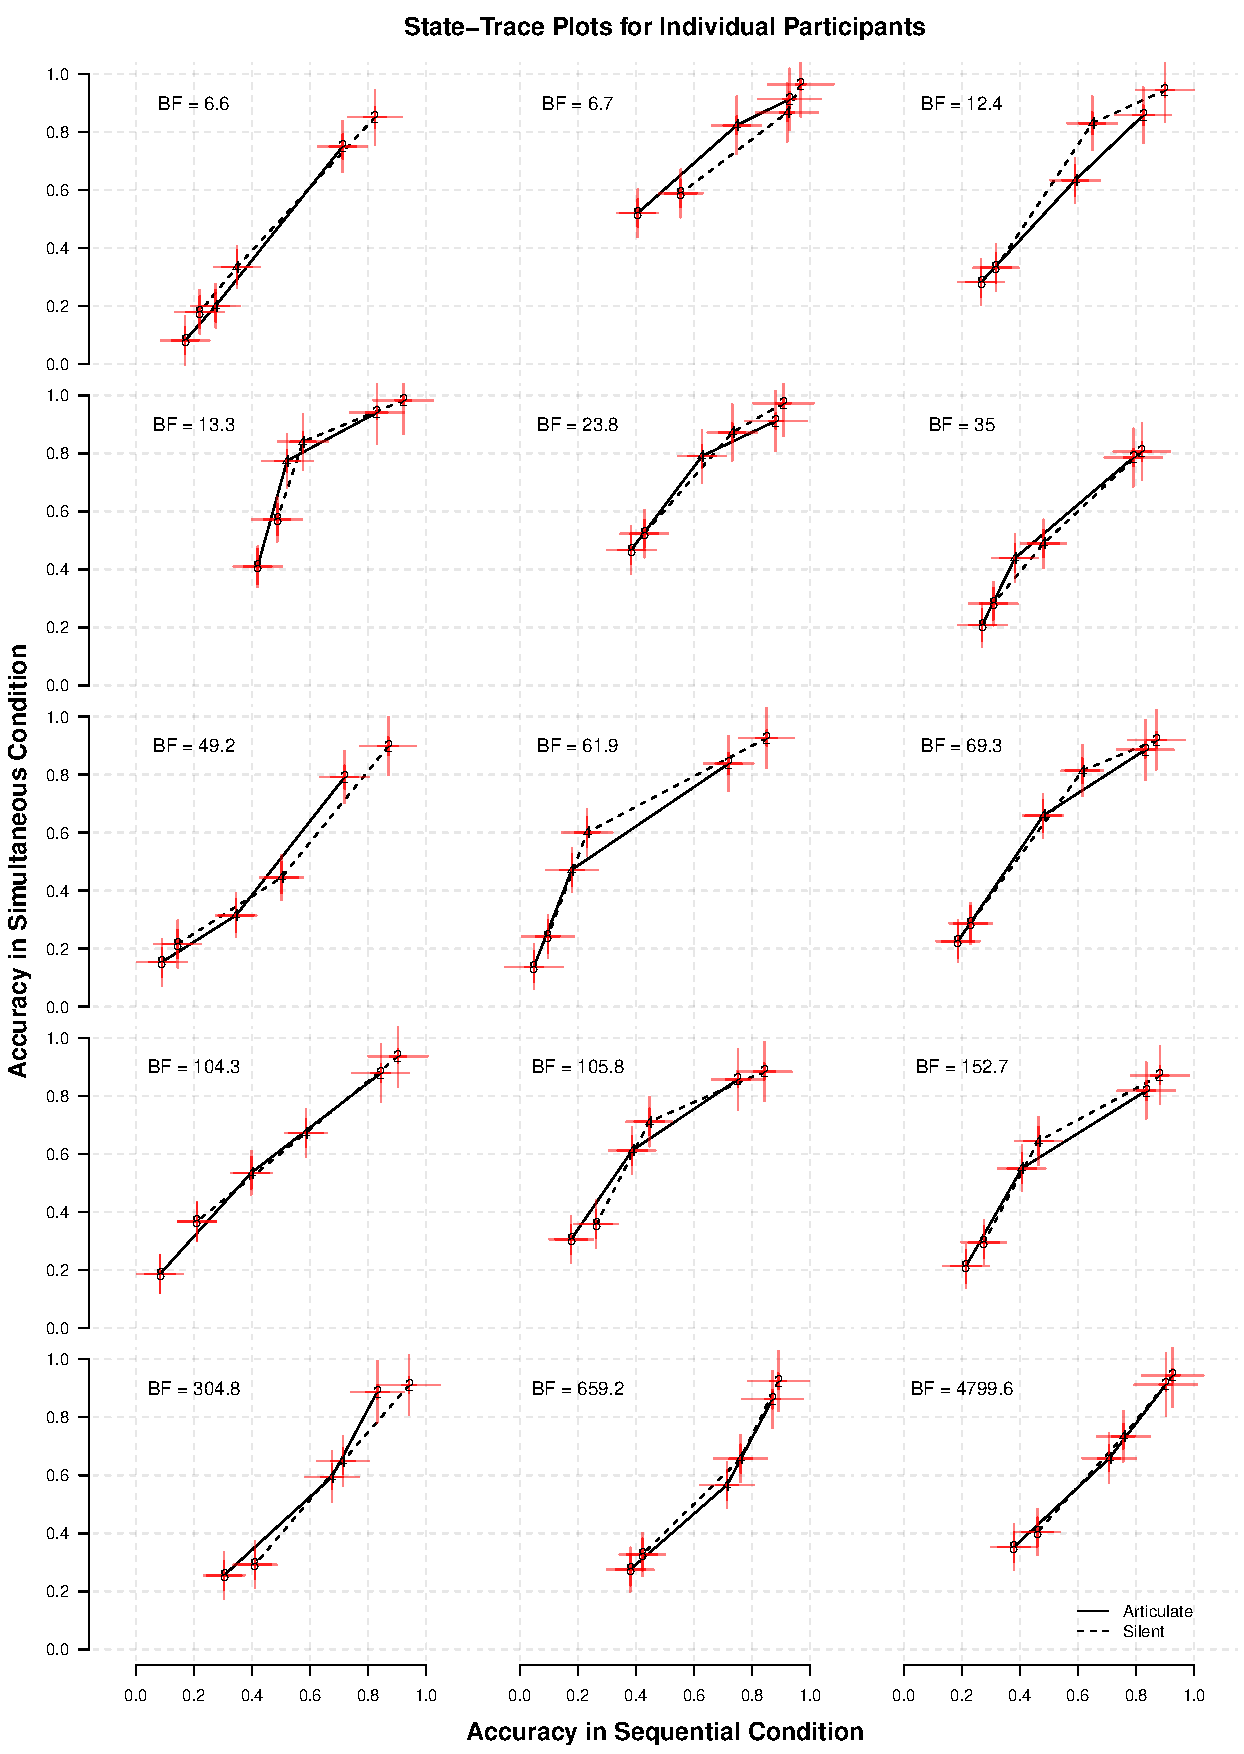
\includegraphics[width=\textwidth]{figures/grid_plot_v2}
	\caption{Individual state-trace plots for the 15 participants. The dependent variables are hit rate minus false alarm rate $d$ for the three set sizes (2, 4, and 8)  and are plotted with standard errors. In the top left corner, individual plot also features the Bayes factor in favor of a monotone ordering of the points over a non-monotone ordering.}

	\label{fig:ST_plots}
\end{figure}

Figure~\ref{fig:ST_plots} shows the state-trace plots for each participant, formed by plotting estimated performance in the simultaneous presentation condition against the performance in the sequential condition. State-trace logic says that more than one latent construct is needed to explain the data to the extent that these points cannot be joined by a single, monotone curve; however, as can be seen from the state-trace plots for all participants, the state-trace plots are strikingly monotone. There does not appear to be any evidence that more than a single latent construct --- (visual) working memory capacity --- is needed, and thus no evidence that verbalization plays a role in performance in this task.

One way to quantify the support for monotonicity in the state-trace plots is to compute Bayes factors that compare the evidence for two hypotheses: first, that the true performance underlying the state-trace plots are ordered the same on both axes (that is, they can be described by a monotone curve), and second, that they are not ordered the same on both axes \citep{Prince:etal:2012}. The Bayes factor is a measure of relative support indicating the degree to which the data change the odds favoring one hypothesis over the other. A Bayes factor of 10, for instance, indicates that the data should change the odds in favor of one hypothesis over the other by a factor of 10. If, before observing the data one was equally disposed to the two hypotheses (a relative odds of 1), then after the data, the favored model would be supported by an odds of $10 \times 1 = 10$.  Here, we discuss the numerical values of the Bayes factors without providing details of their calculation. We refer the reader to \citet{Prince:etal:2012} for technical details, and to the supplement to this article for details of how the Bayes factors were computed \citep[see also][]{Davis-Stober:etal:inpress}.

In addition to the state-trace plots for each participant, Figure~\ref{fig:ST_plots} also contains the Bayes factor favoring a monotone ordering of the points over a non-monotone one. The Bayes factors uniformly favor the monotone ordering of the points. The Bayes factors range from about 7 to almost 5000. These data do not appear to provide any evidence for a deviation from monotonicity.